\newcommand{\pictureslideb}[3]{
	\begin{frame}{#1}
		\begin{center}
			#3
			
			\vspace{6pt}
			
			\includegraphics[height=0.6\textheight]{#2}
		\end{center}
	\end{frame}
}

\newcommand{\pictureslide}[2]{
	\begin{frame}{#1}
		\begin{center}
			\includegraphics[height=0.6\textheight]{#2}
		\end{center}
	\end{frame}
}

\part{What was the first computer?}
\frame{\partpage}

\pictureslideb{Antikythera Mechanism ($\sim$150 BC)}{antikythera}{First mechanical computer?}
\pictureslideb{Jacquard Loom (1804)}{jacquard}{First programmable machine in modern age}
\pictureslideb{Babbage's Difference and Analytical Engines (1837)}{difference_engine}{First mechanical computer in modern age}
\pictureslideb{Colossus (1943)}{colossus}{First programmable electronic computer}
\pictureslideb{ENIAC (1946)}{eniac}{First general-purpose computer}
\pictureslideb{Manchester Small-Scale Experimental Machine (1948)}{manchester}{First stored program computer}
%\pictureslideb{EDSAC (1949)}{edsac}{Many firsts in mathematics and science}
\pictureslideb{TRADIC (1949)}{tradic}{First transistor computer}
\pictureslideb{PDP-1 (1959)}{pdp1}{Influenced ``hacker culture''}
\pictureslideb{Datapoint 2200 (1970)}{datapoint2200}{First microcomputer}
\pictureslideb{Commodore VIC 20 (1980)}{vic20}{First computer to sell 1 million units}
\pictureslideb{IBM Personal Computer Model 5150 (1981)}{ibm_5150}{Precursor to the modern PC}

\part{Electronic computer technologies}
\frame{\partpage}

\pictureslide{Vacuum tubes (valves)}{vacuum_tubes}
\pictureslide{Transistors}{transistors}
\pictureslide{Integrated circuits (ICs)}{6502}

\begin{frame}
    \begin{tabular}{|c|l|r|}
        \hline
        1943 & Colossus & 1700 valves \\\hline\pause
        1946 & ENIAC & 20000 valves \\\hline\pause
        1949 & TRADIC & 800 transistors \\\hline\pause
        1959 & PDP-1 & 2700 transistors \\\hline\pause
        1975 & MOS 6502 & 3510 transistors \\\hline\pause
        1979 & Intel 8088 & 29000 transistors \\\hline\pause
        1998 & Intel Pentium II & 7.5 million transistors \\\hline\pause
        2016 & Intel Core i7 Broadwell-E & 3.2 billion transistors \\\hline\pause
        2020 & Apple A14 & 11.8 billion transistors \\\hline\pause
        2020 & Nvidia GeForce RTX 3080 & 28 billion transistors \\\hline
    \end{tabular}
\end{frame}

\begin{frame}
    \begin{center}
        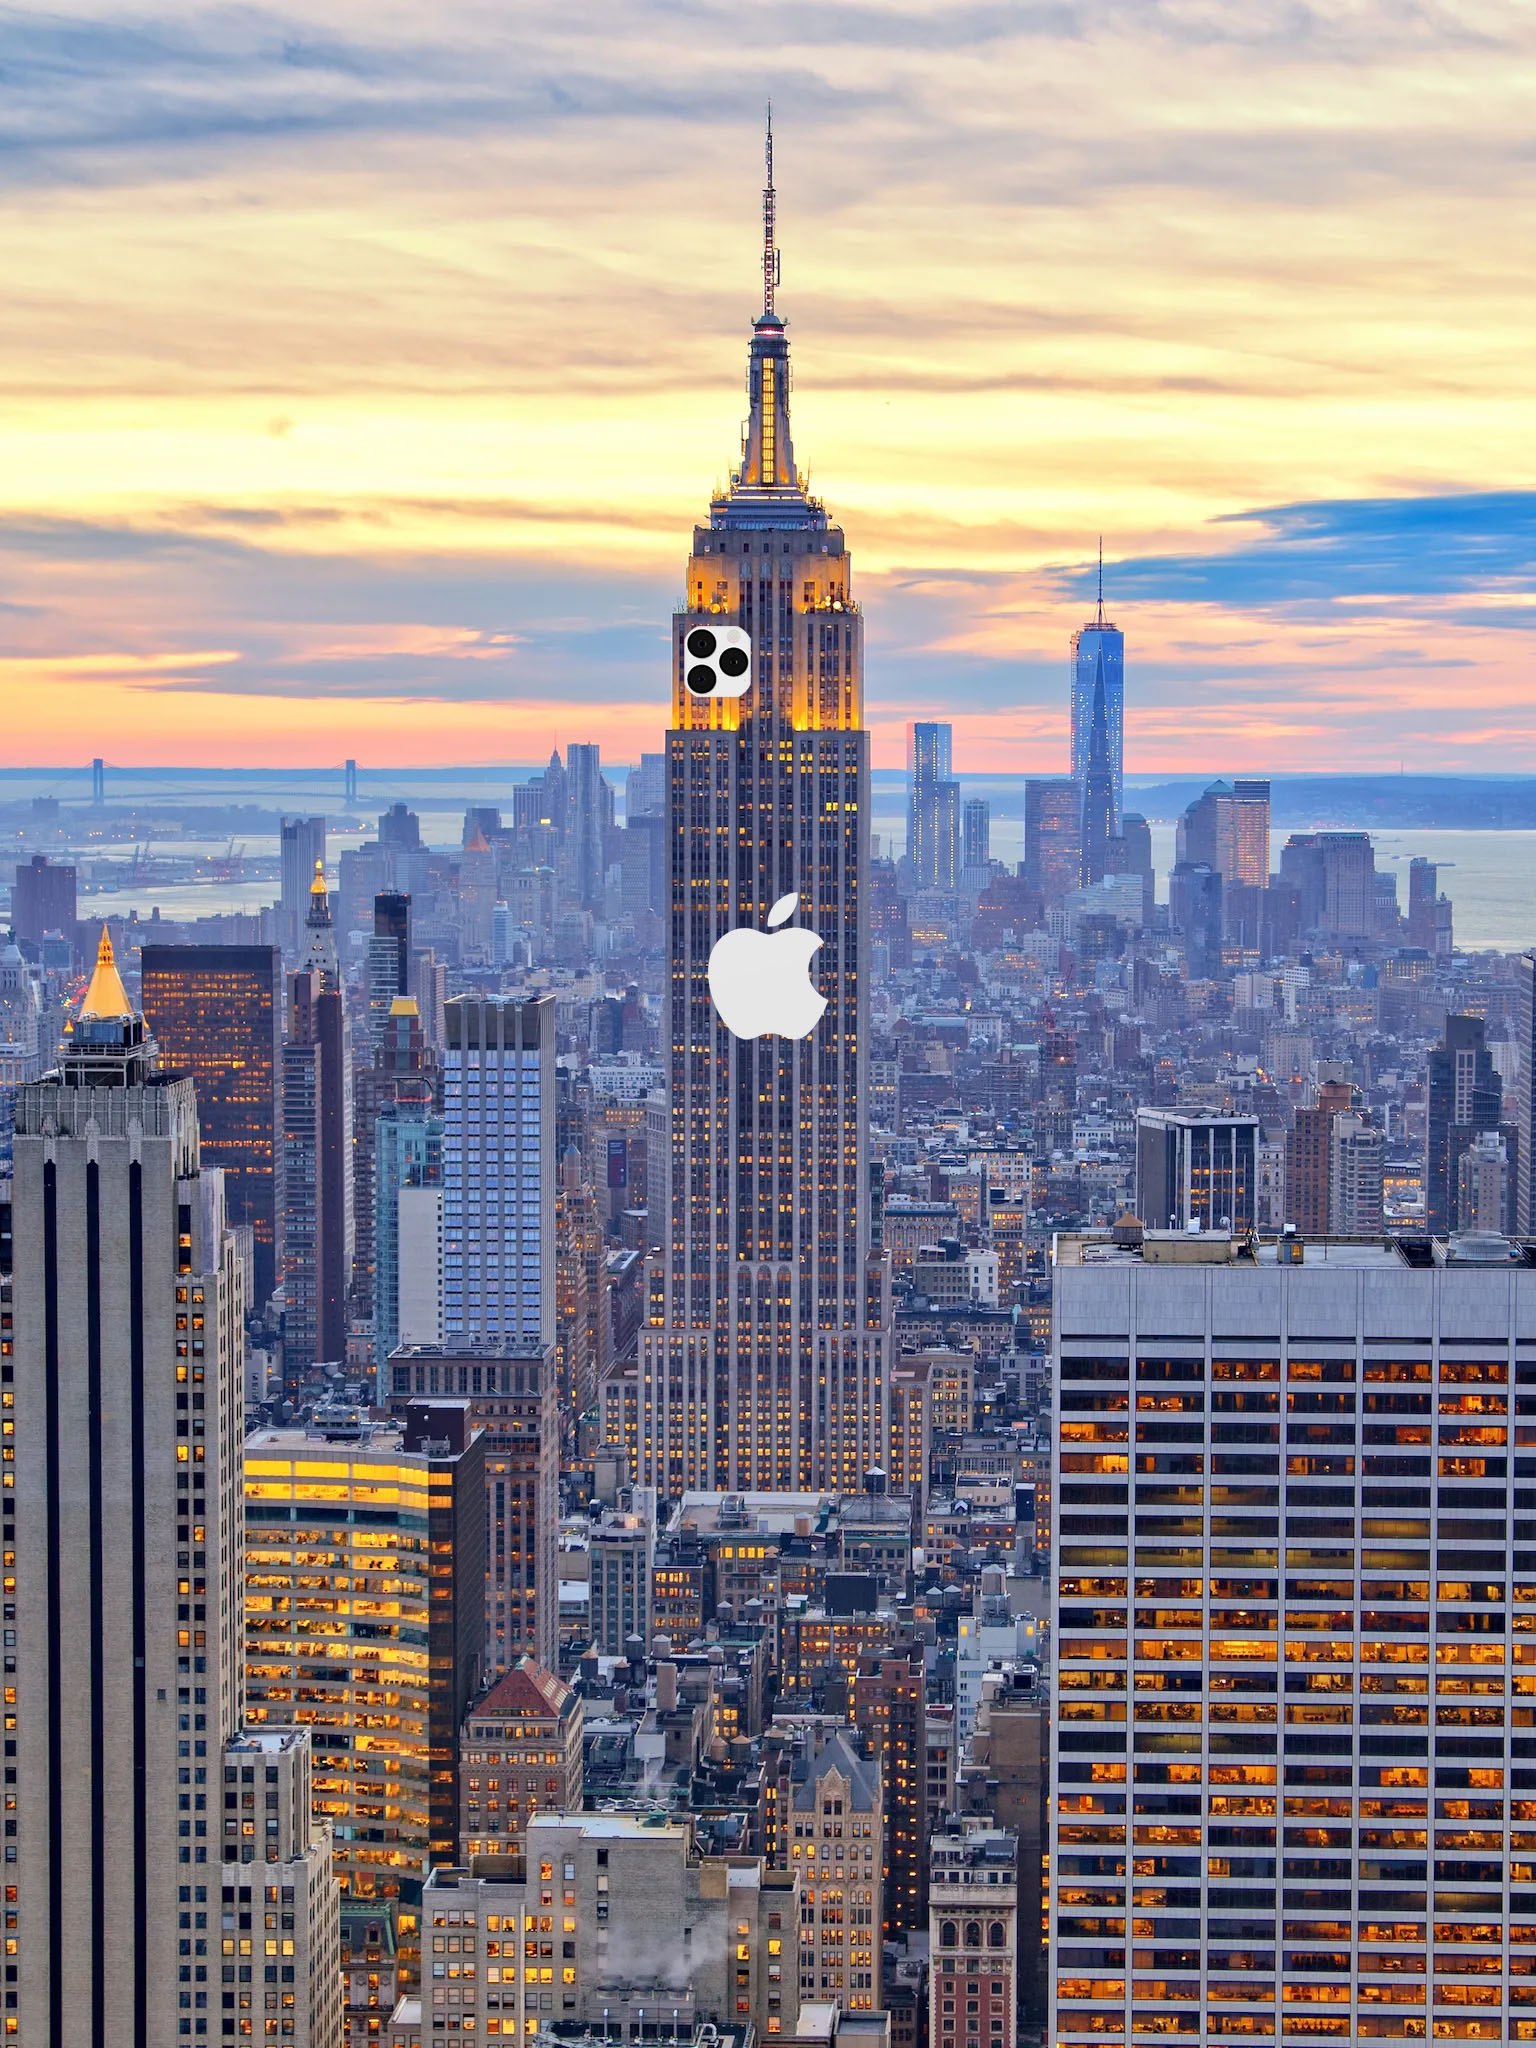
\includegraphics[height=0.8\textheight]{empire-state-iphone}
    \end{center}
\end{frame}

\part{What was the first computer game?}
\frame{\partpage}

\pictureslideb{Cathode Ray Tube Amusement Device (1948)}{crt}{First interactive electronic game}
\pictureslideb{Chess AI on the Ferranti Mark I (1951)}{ferranti}{First chess program}
\pictureslideb{Bertie the Brain (1950)}{bertie}{First computer game with a visual display}
\pictureslideb{OXO (1951)}{oxo}{First game with visuals on a general-purpose computer}
\pictureslideb{Tennis for Two (1959)}{tennis}{First to be created purely for entertainment}
\pictureslideb{SpaceWar! (1962)}{spacewar}{First widely available game, inspired first arcade games}
\pictureslideb{Pong (1972)}{pong}{First commercially successful game}

\part{What was the first games console?}
\frame{\partpage}

\pictureslideb{The Brown Box (1967)}{brownbox}{First prototype console}
\pictureslideb{Magnavox Odyssey (1972)}{magnavox}{First commercial console}

